% Load packages
\documentclass[12pt,fleqn]{article}
\usepackage{fullpage}
\usepackage{setspace}
\usepackage{amssymb,amsthm,mhchem}
\usepackage{pbyp}
\usepackage[commandnameprefix=always]{changes}
\usepackage{hyperref}


\onehalfspacing

%\setlength{\parindent}{0pt} % No indents

\begin{document}
\begin{flushleft}
Manuscript Number: CMAME-D-24-01642

Title: Phase-field analysis for brittle fracture in ferroelectric materials with flexoelectric effect

Author(s): Yu Tan; Yong Zhang; Zhaoyi Liu; Takahiro Shimada; Xiangyu Li; Jie Wang    
\end{flushleft}
\begin{flushleft}
Dear Professor Laura De Lorenzis,
\end{flushleft}

Thank you very much for your email on 3 July. We appreciate all the comments from the reviewer. We revise the manuscript according to reviewer’s comments and suggestions. We think the quality of the revised manuscript has been improved greatly. Attached please find the revised manuscript, the replies to the reviewer's comments, and the revised manuscript with tracked changes.

Please feel free to contact me if you need further information. Thank you very much for your consideration.

\begin{flushleft}
Sincerely yours,

~ 

Chang Liu

~

Assistant Professor

School of Mechanics and Aerospace Engineering, 

Southwest Jiaotong University

Chengdu, Sichuan 611756, China

Email: \href{mailto:lc@swjtu.edu.cn}{lc@swjtu.edu.cn}
\end{flushleft}

\newpage
\begin{flushleft}
    \textbf{Replies to reviewer’s comments}
    \vspace{1em} 
    \hrule
    \vspace{1em} 
    \textbf{Point-by-point Reply to Reviewer1}
    \vspace{1em} 
    \hrule
    \vspace{1em} 
\end{flushleft}
\begin{question}{\QuestionRevA{General}}\label{R1:general}
I think this is an interesting paper that is worth publishing in CMAME. I have the following revisions that I believe should be made.
\end{question}

\begin{response}
First, we express our sincere gratitude to you for your careful evaluation and useful comments to improve the quality of the manuscript. We answer all your comments and revise the manuscript accordingly as follows.
\end{response}

% First question by reviewer 1
\begin{question}{\QuestionRevA{Q1}}\label{R1:Q1}
In Eq. 7, the dielectric permittivity should be the permittivity of free space as the permittivity of the material is already accounted for in the Landau part of the free-energy.
\end{question}

\begin{response}
Thank you very much for your suggestion. For ferroelectric materials with perovskite crystal structure, spontaneous polarization appears when the crystal changes from cubic phase to tetragonal phase. According to Y. L. Li’s (APL, 81.3, 427-429, 2002) and J. Wang’s (\href{ https://hdl.handle.net/1783.1/2614}{\textcolor{blue}{\underline{Ph. D thesis, 2006}}}; JAP, 105.1, 2009) research, the cubic paraelectric phase is used as the background material in the phase-field model. Spontaneous polarizations associated with spontaneous strains are embedded within the background material. Thus, the total polarization $\mathbf{P}^t$ can be divided into two components: the spontaneous polarization $\mathbf{P}$ and the electric field induced polarization $\mathbf{P}^i$. The spontaneous polarization is used as the order parameter in the phase field model, as presented in Eq.(2) of the manuscript. For simplicity, $\mathbf{P}^i$ is linearly proportional to the electric field. In this case, the electric displacement $\mathbf{D}$ is
\begin{equation*}
    \mathbf{D}=\varepsilon_0 \mathbf{E}+\mathbf{P}^t=\varepsilon_0 \mathbf{E}+\mathbf{P}^i+\mathbf{P}=\varepsilon_0 \varepsilon_r \mathbf{E}+\mathbf{P}
\end{equation*}
in which $\varepsilon_r$ represents the relative dielectric constant of the background material. Therefore, $\mathbf{K}$ should be the dielectric coefficient of the background material in Eq.(7) of the manuscript.

To clarify this, we have added the following explanation in the revised manuscript:
\begin{enumerate}
    \item After Eq.(1),
    \begin{revised}
        …, where $\varepsilon=\frac{1}{2}\left[ \nabla u+(\nabla u)^T\right]$ is the total strain, … and $\mathbf{P}$ represents the displacement vector, electric potential, and \textcolor{blue}{spontaneous} polarization vector, respectively. 
    \end{revised}
    \item After Eq.(8) of the revised manuscript,
    \begin{revised}
        ... where $\mathbf{K}$ represents the dielectric coefficient \textcolor{blue}{of the background material [44, 45]}, ...
    \end{revised}
\end{enumerate}

\end{response}

% First question by reviewer 2
\begin{question}{\QuestionRevA{Q2}}\label{R1:Q2}
How different parts of the energy can be degraded in order to reproduce impermeable, permeable, and semi-permeable crack-face boundary conditions has been discussed in Wilson et al. (2013) Int. J. Fract. 183, 135-153. I think this is a useful reference to include.
\end{question}

\begin{response}
We highly appreciate you for your important comments. We appreciate your suggestion to include the reference to Wilson et al. (2013) from the International Journal of Fracture. We agree that this reference provides valuable insight into the energy degradation for different electrical boundaries of the crack surface. 

According to your suggestion, we have added the reference  before Eq.(15) in the revised manuscript:
\begin{revised}
    … there are two classical extreme assumptions, namely electrically permeable and impermeable boundary conditions [\textcolor{blue}{49, 50}]. Under the permeable boundary condition, ...  
\end{revised}
(Ref. 50 is the research by Wilson et al.)
\end{response}

% Second question by reviewer 2
\begin{question}{\QuestionRevA{Q3}}\label{R1:Q3}
In Eq. 18, D should be minus the derivative of the enthalpy with respect to E.
\end{question}
\begin{response}
Thank you for pointing out the issue with Eq. (18). We apologize for the oversight in the equation. We have corrected it in the revised manuscript to ensure accuracy. As you can see in the response \cref{R2:Q2}
\end{response}

\begin{question}{\QuestionRevA{Q4}}\label{R1:Q4}
Ginzburg is misspelled prior to Eq. 22.
\end{question}

\begin{response}
Thanks for your carefully reading and constructive comments. We are sorry for the typo. We have addressed this issue in the revised manuscript.
\begin{revised}
... is governed by the time-dependent \textcolor{blue}{Ginzburg} Landau equation:
\end{revised}
\end{response}

\begin{question}{\QuestionRevA{Q5}}\label{R1:Q5}
Eq. 24 is ad hoc. I don't understand why this is done since the experiments of Park and Sun are reasonably well explained using permeable crack face boundary conditions. At the very least I think that one of the simulations should be rerun with the consistent driving force for the permeable boundary condition case to illustrate if there is any difference, and how significant such a difference is if one exists.    
\end{question}

\begin{response}
Thank you very much for your constructive comments. In Park and Sun’s search (JACS, 78.6, 1475-1480, 1995), the specimen is immersed in a tub filled with silicone oil. Thus, in their experiment, the boundary conditions of the insulated crack surface were established. In our simulation, we assumed the crack is filled with air. According to Wang's study (EFM, 77.18, 3658-3669, 2010), this can be regarded as an electrically impermeable crack. Since the main topic of our discussion is about the influence of the flexoelectric effect, we chose to focus on the electrically impermeable crack for simplicity.

We appreciate the opportunity to further enhance our work. We have included a brief comparison of the fracture process with the flexoelectric effect, considering cracks parallel and perpendicular to the crack under electrically impermeable conditions. Our computational results indicate that the flexoelectric effect can induce asymmetric fracture toughness in ferroelectric materials, regardless of whether the cracks are electrically permeable or impermeable.

In the revised manuscript, the following changes are made:
\begin{enumerate}
    \item  On page 24 of the revised manuscript:
    \begin{revised}
    The complete evolution process of the domain structure and crack path is presented in Video S3. \textcolor{blue}{For the permeable crack, the temporal evolution of domain structure and crack path are like those in Figure 5, as shown in Figure S1 (a)-(d).}
    \end{revised}
    \item On page 26 of the revised manuscript: \begin{revised}
        The complete spatial and temporal evolution of the domain structure and crack path is presented in Video S4. \textcolor{blue}{As depicted in Fig. S1 (e)-(h), the polarization switched zone is significantly thinner for electrically permeable cracks. The temporal evolution of the domain and crack path are similar to those in Figure 6. However, they occur later and do not form diamond structures.}
    \end{revised}
    \item  On page 26 of the revised manuscript:
    \begin{revised}
        ... effectively increasing the material's fracture toughness. \textcolor{blue}{Analogous to the behavior of electrically impermeable cracks, the flexoelectric effect can also} \textcolor{blue}{influence crack extension in electrically permeable cracks, as illustrated in Figure S2. When the propagation direction is aligned with the polarization direction, fracture occurs earlier. Conversely, when the propagation direction is opposite to the polarization direction, crack growth is delayed.} Thus, the flexoelectric effect can lead to asymmetric fracture toughness of ferroelectric materials \textcolor{blue}{for both the electrically impermeable and permeable crack}. This numerical result ...
    \end{revised}
    \item On page 35 of the revised manuscript:
    \begin{revised}
        Video S8 displays the complete spatial and temporal evolution of the domain structure and crack path. \textcolor{blue}{For electrically permeable cracks, the electric field remains continuous on both sides of the crack, which ensure a uniform electric field in the ferroelectric material. During crack propagation, the polarization maintains a single domain state aligned with the electric field direction. Nevertheless, under the influence of the flexoelectric effect, the crack path still undergoes deflection, as presented in Figure S3. When the initial polarization is directed downward, a slight upward deflection occurs in the crack path. Conversely, when the initial polarization is directed upward, the crack path deflects downward.}
    \end{revised}
    \item On page 38 of the revised manuscript:
    \begin{revised}
        … regardless of whether the initial polarization is directed upward or downward. \textcolor{blue}{Similar results can also be observed in electrically permeable cracks, as shown in Figure S4.} These simulation results are consistent with experimental observations, …
    \end{revised}
    \item  Following figures are added in the supplementary materials:
    \begin{figure}
    \centering
    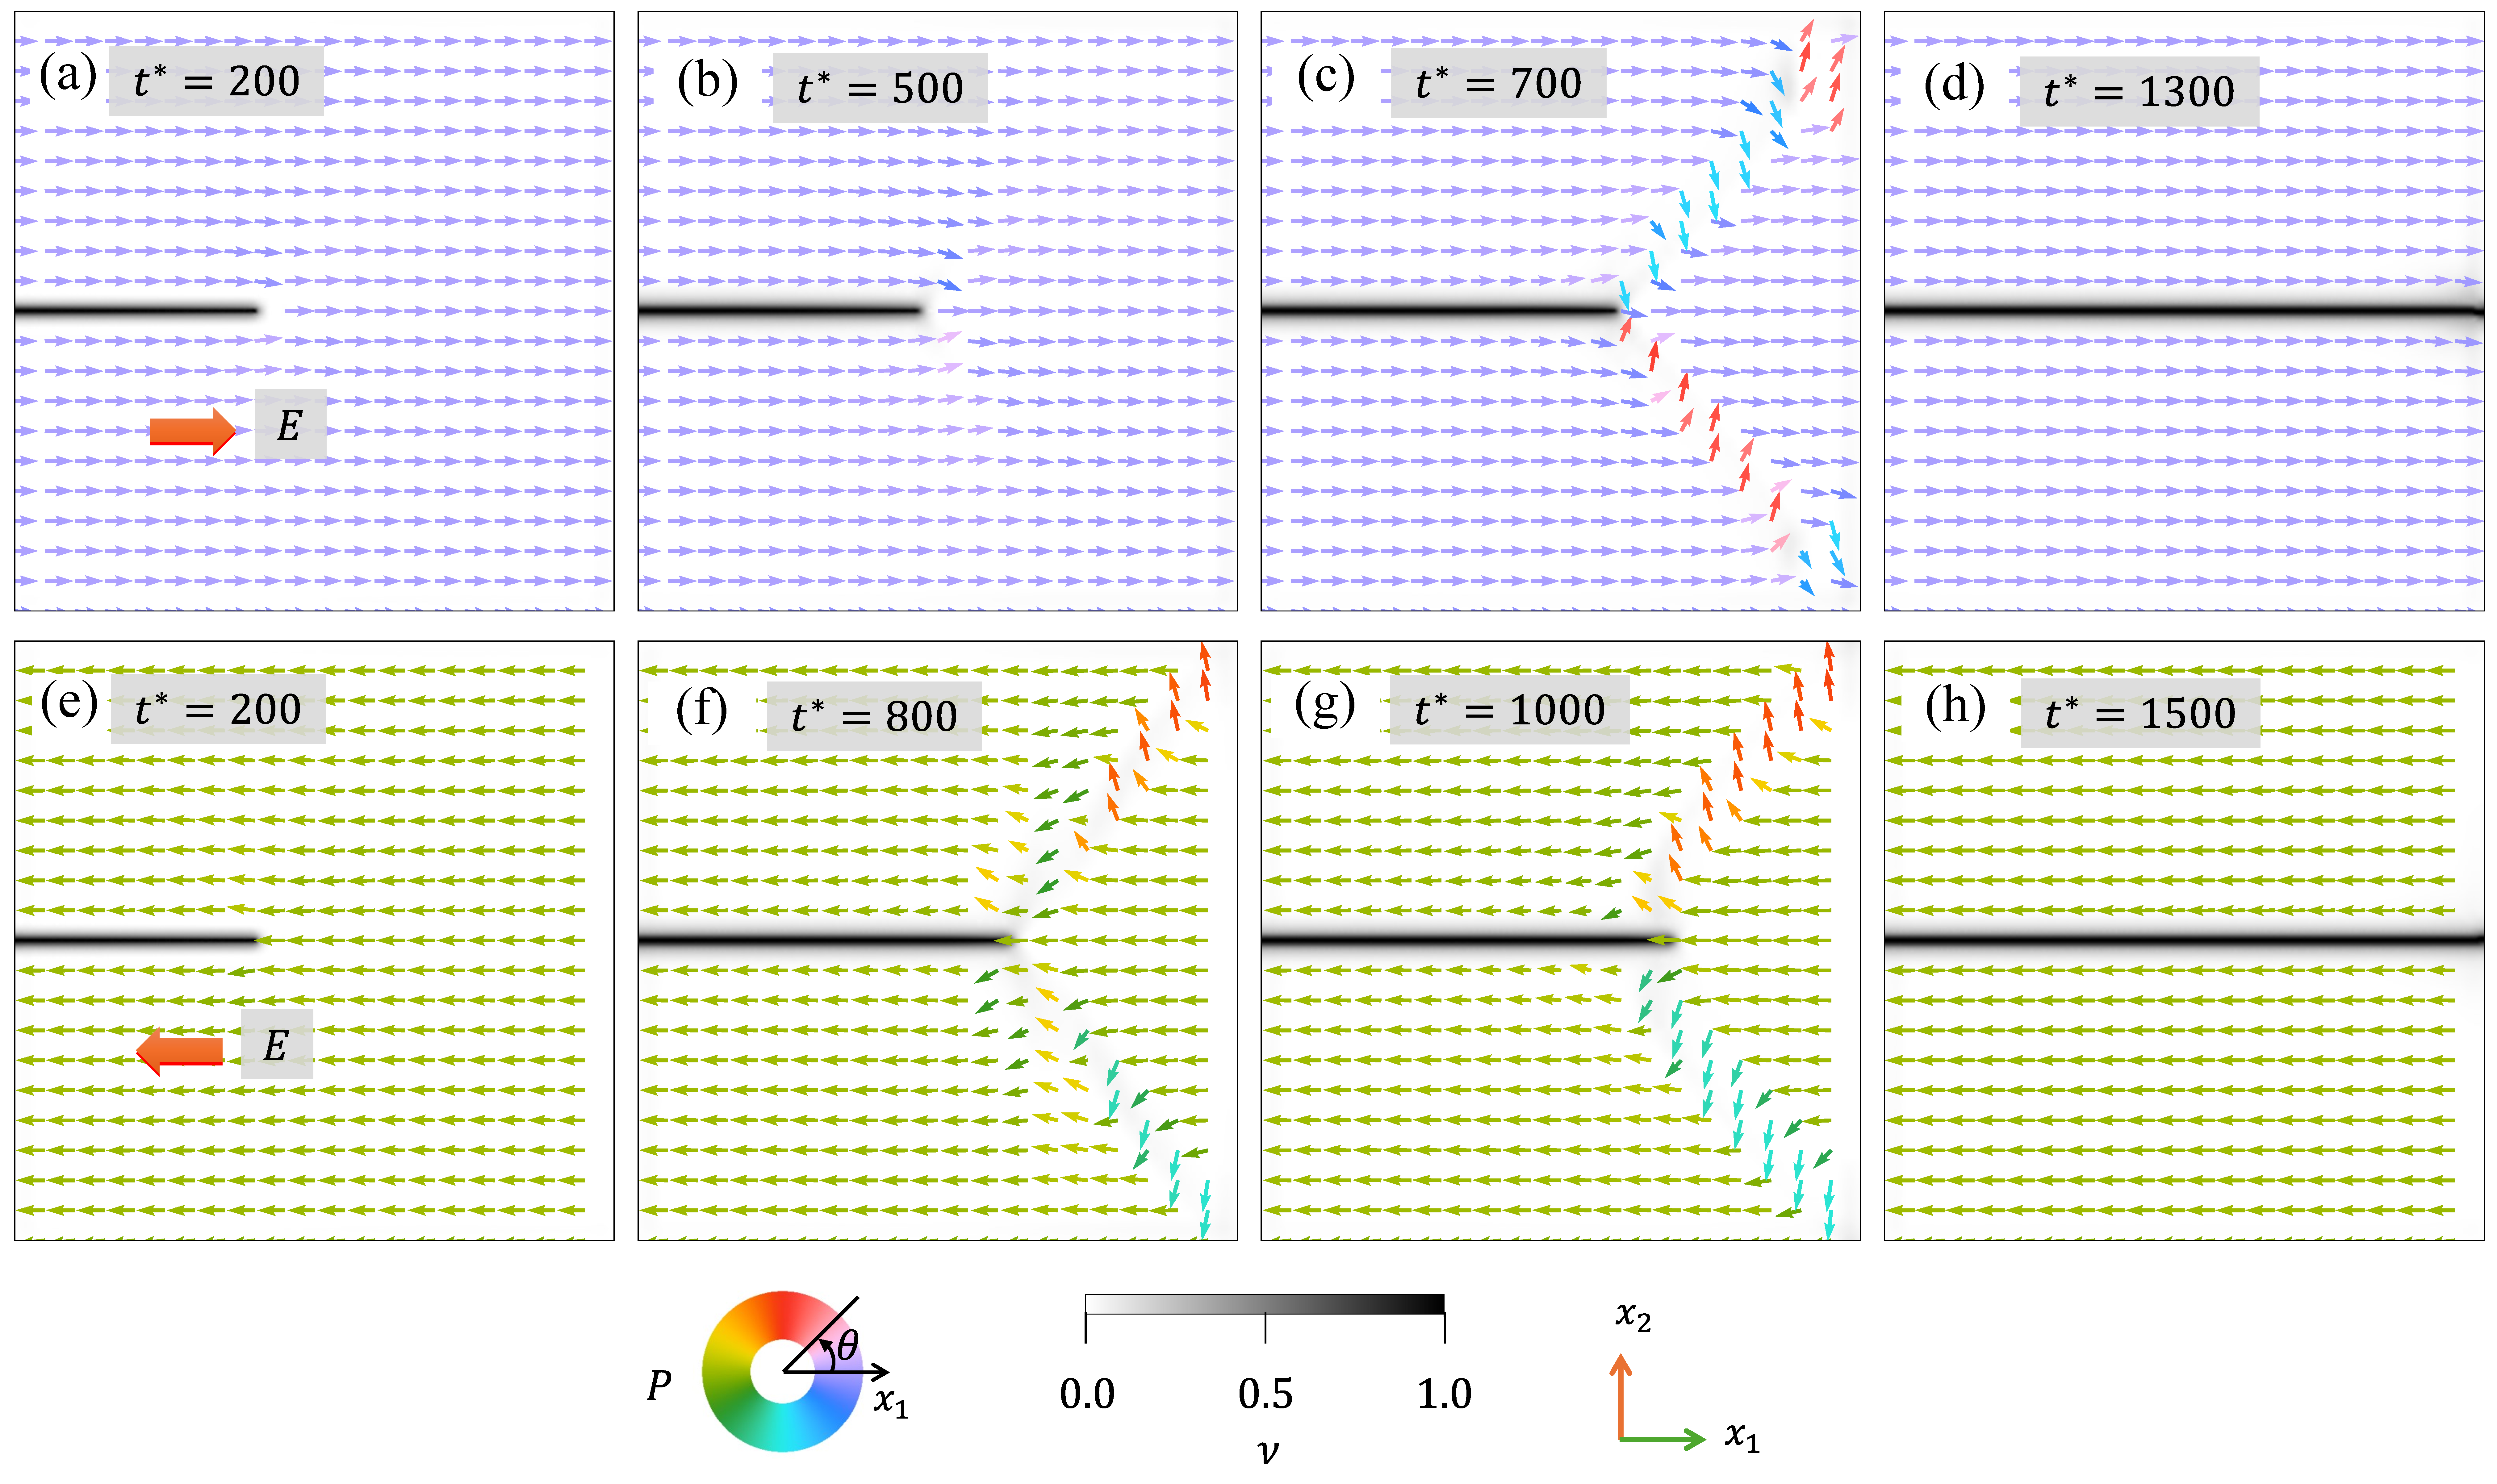
\includegraphics[width=\linewidth]{FigS1.pdf}
    \caption{The temporal evolution of crack and polarization domain: (a)-(d) crack propagates along the polarization direction, (e)-(h) crack direction opposite to the polarization. The grayscale maps illustrate the spatial distribution of the fracture order parameter $\nu$. The arrows indicate the orientation and magnitude of the polarization vectors. The flexoelectric effect is considered in this figure. } \label{figS1}
\end{figure}
\begin{figure}
    \centering
    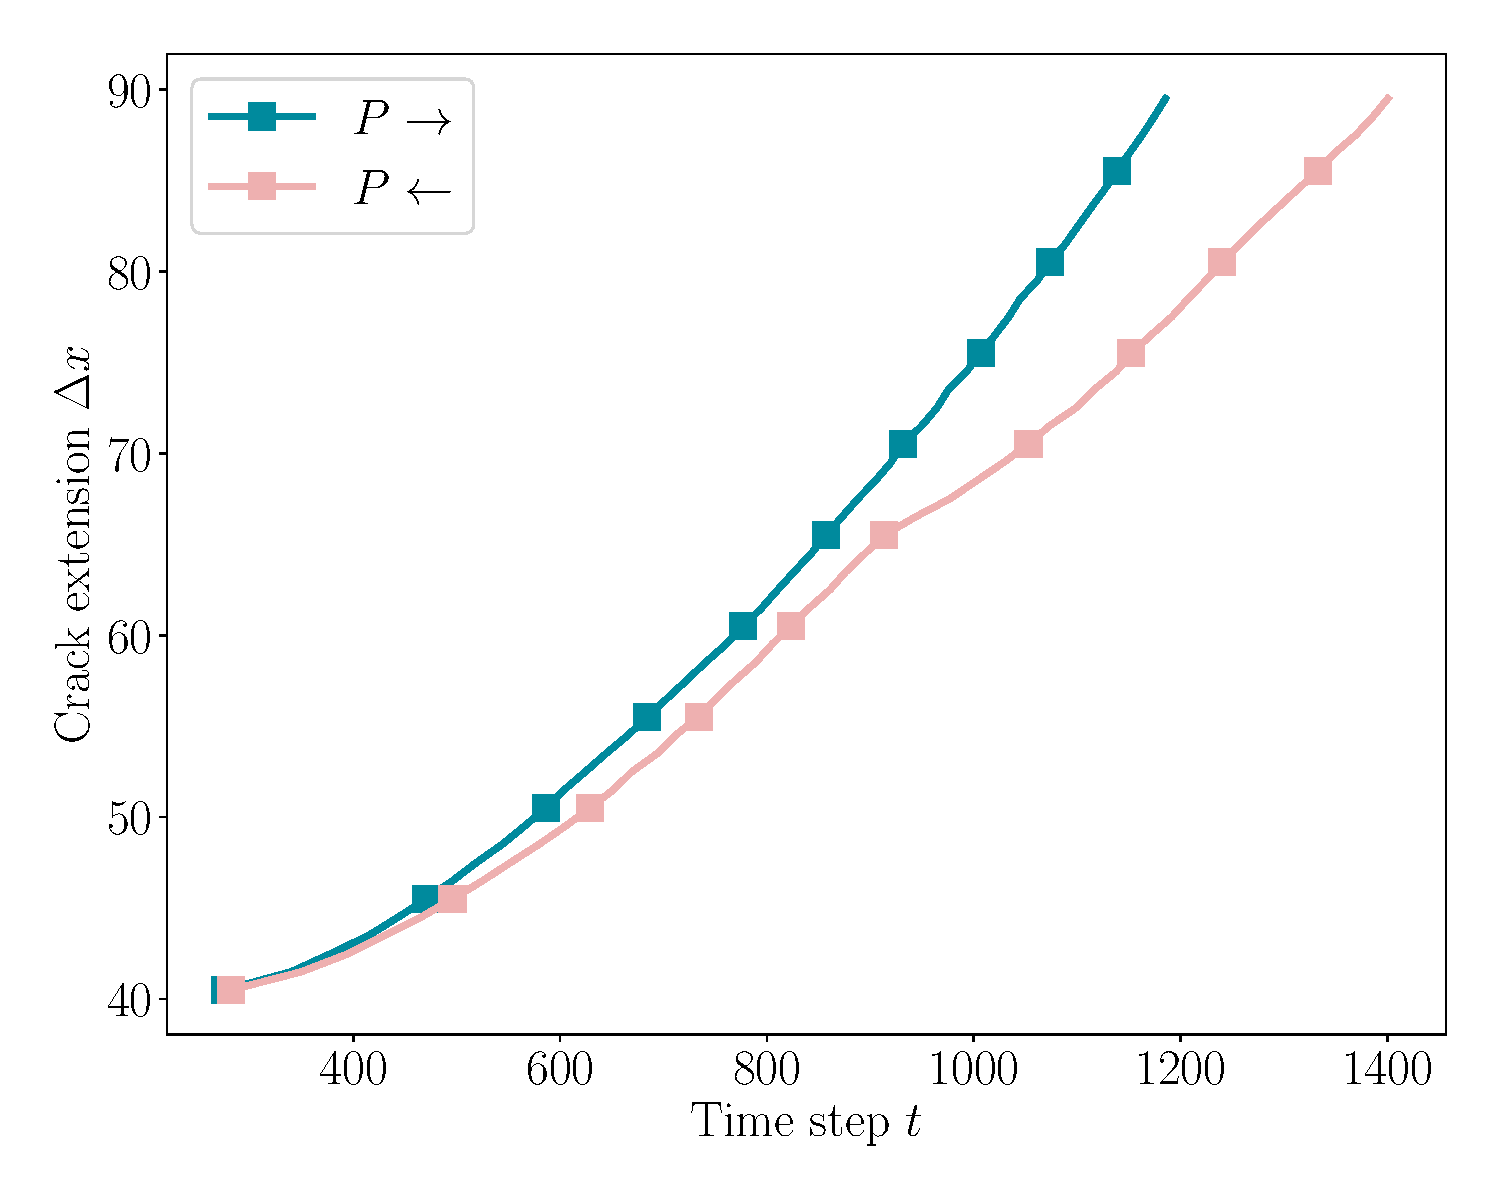
\includegraphics[width=0.55\linewidth]{FigS2.pdf}
    \caption{The change in crack extension length over time step $t$. Arrows in the figure indicate the direction of initial polarization.} \label{figS2}
\end{figure}

\begin{figure}
    \centering
    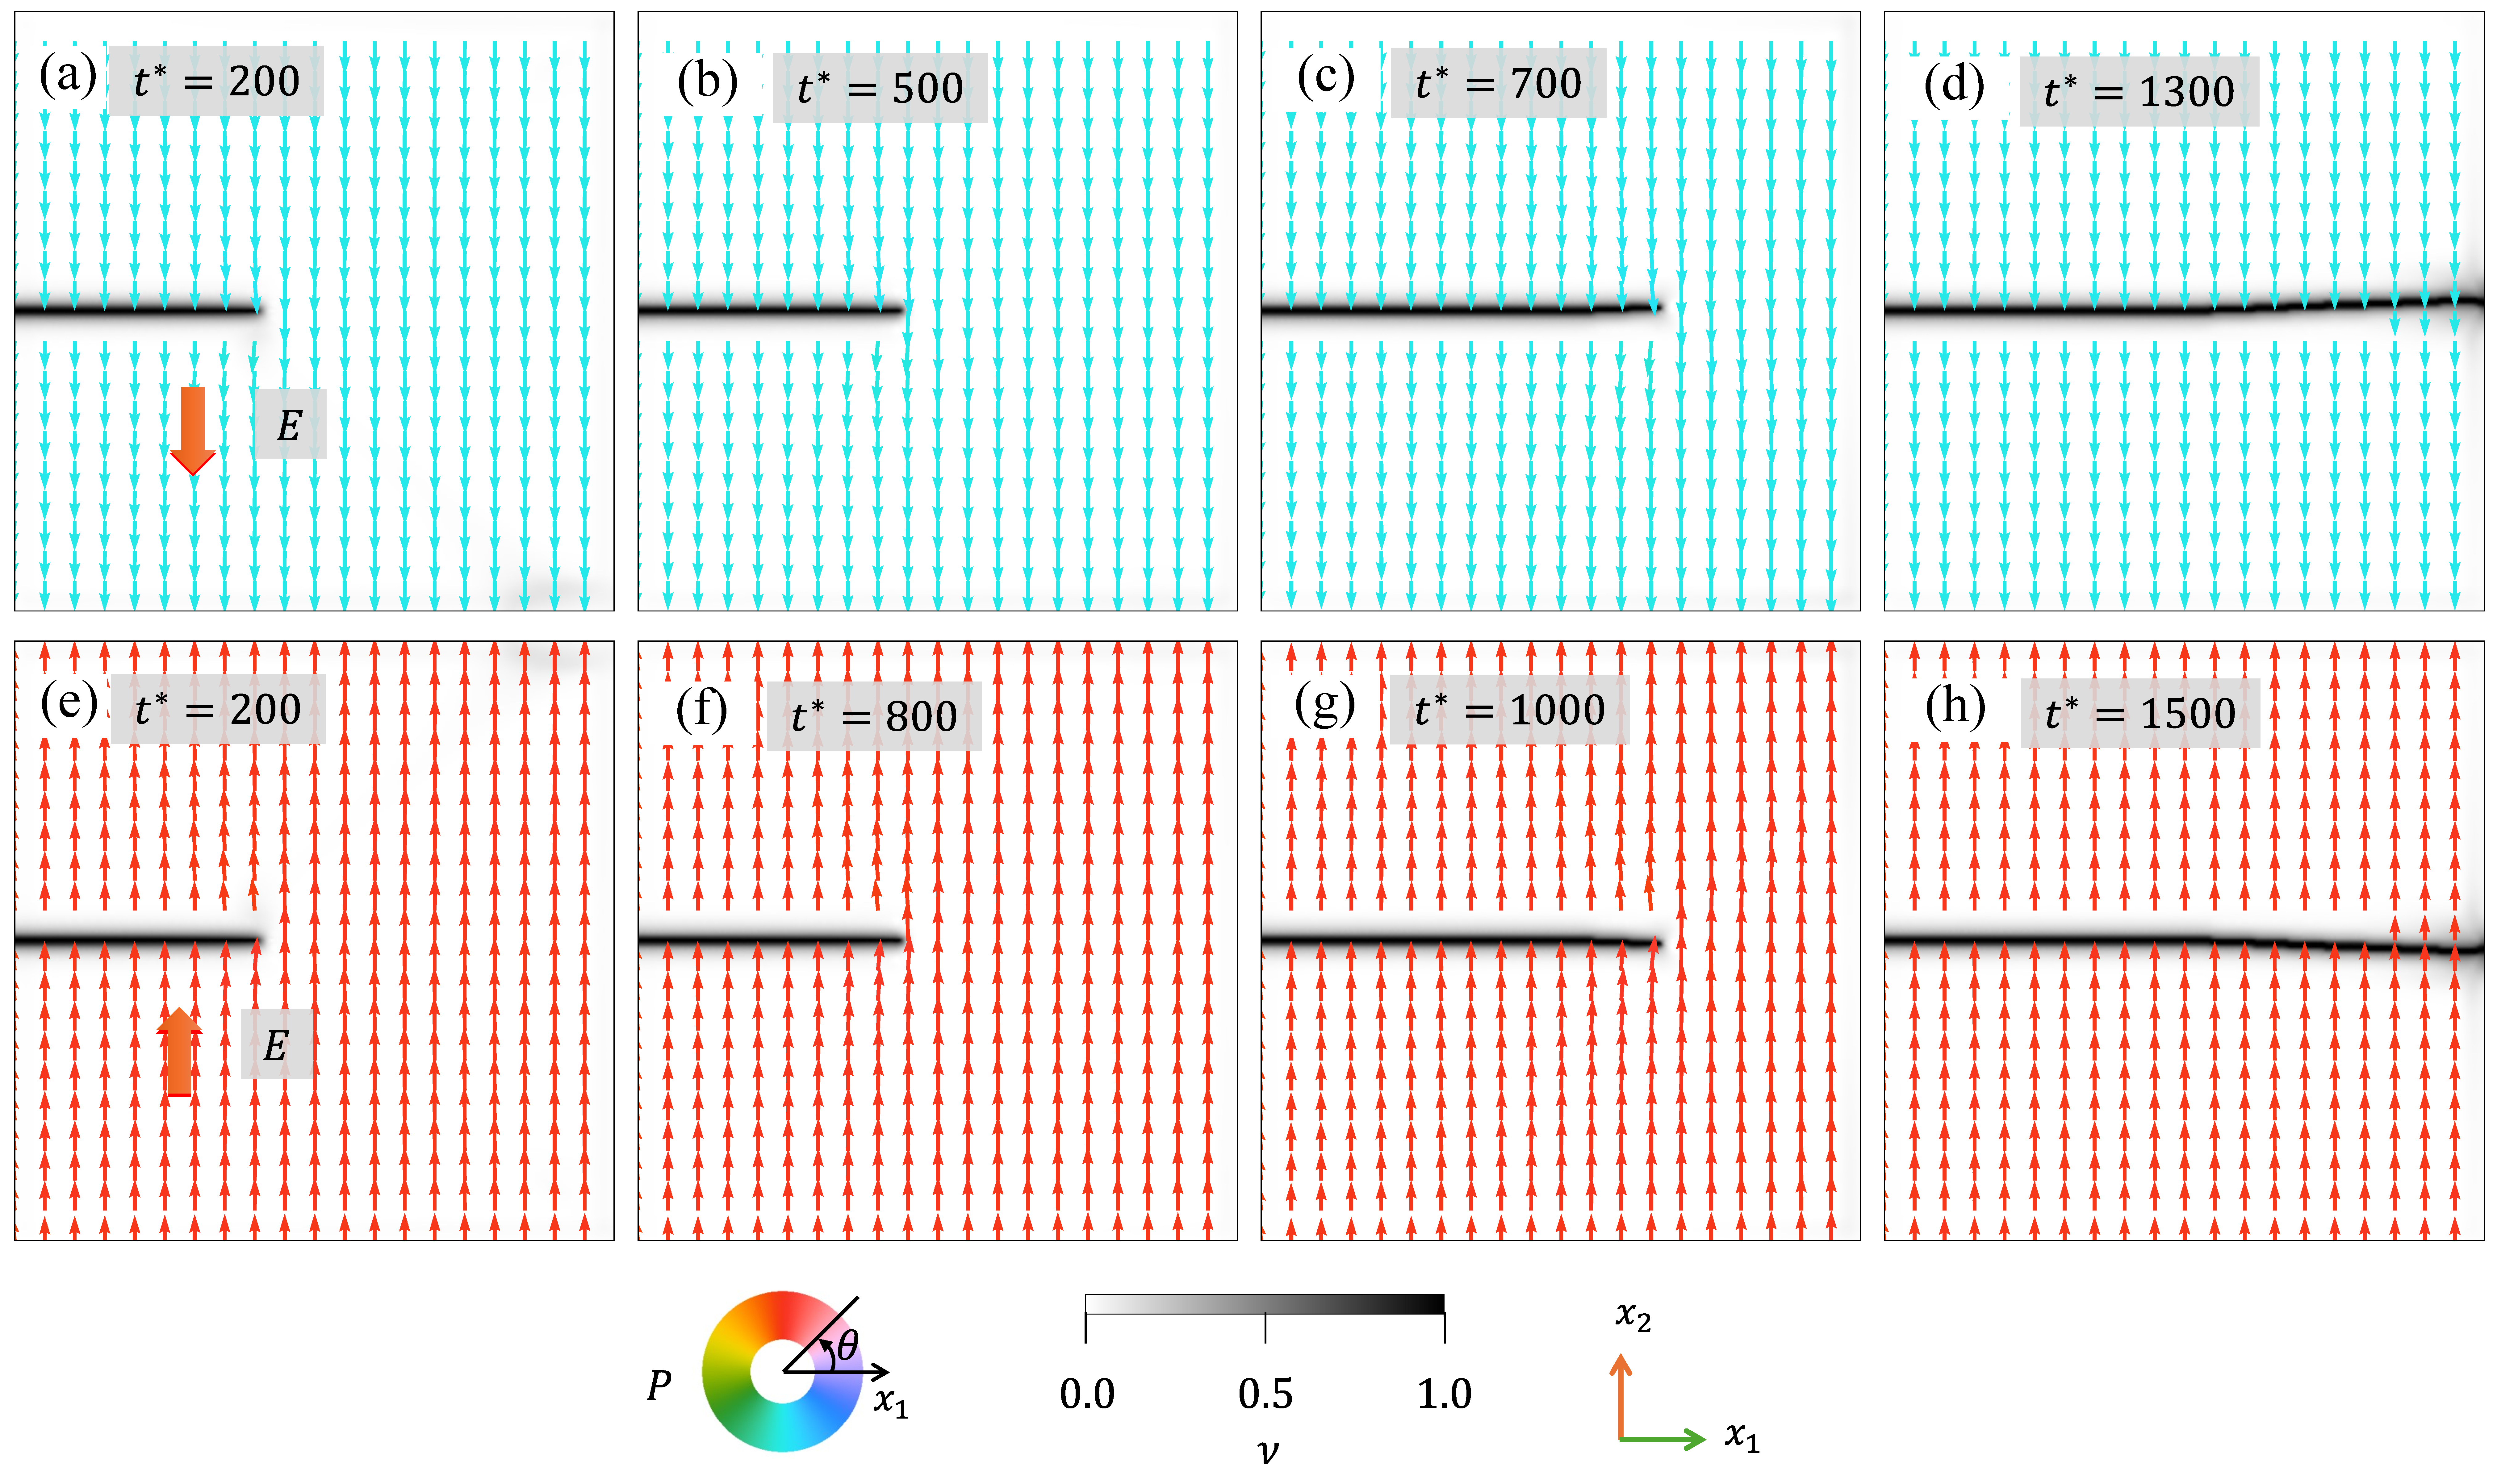
\includegraphics[width=\linewidth]{FigS3.pdf}
    \caption{The temporal evolution of crack and polarization domain: (a)-(d) initial polarization is opposite to the $x_2$-direction, (e)-(h) initial polarization is along the $x_2$-direction.} \label{figS3}
\end{figure}

\begin{figure}
    \centering
    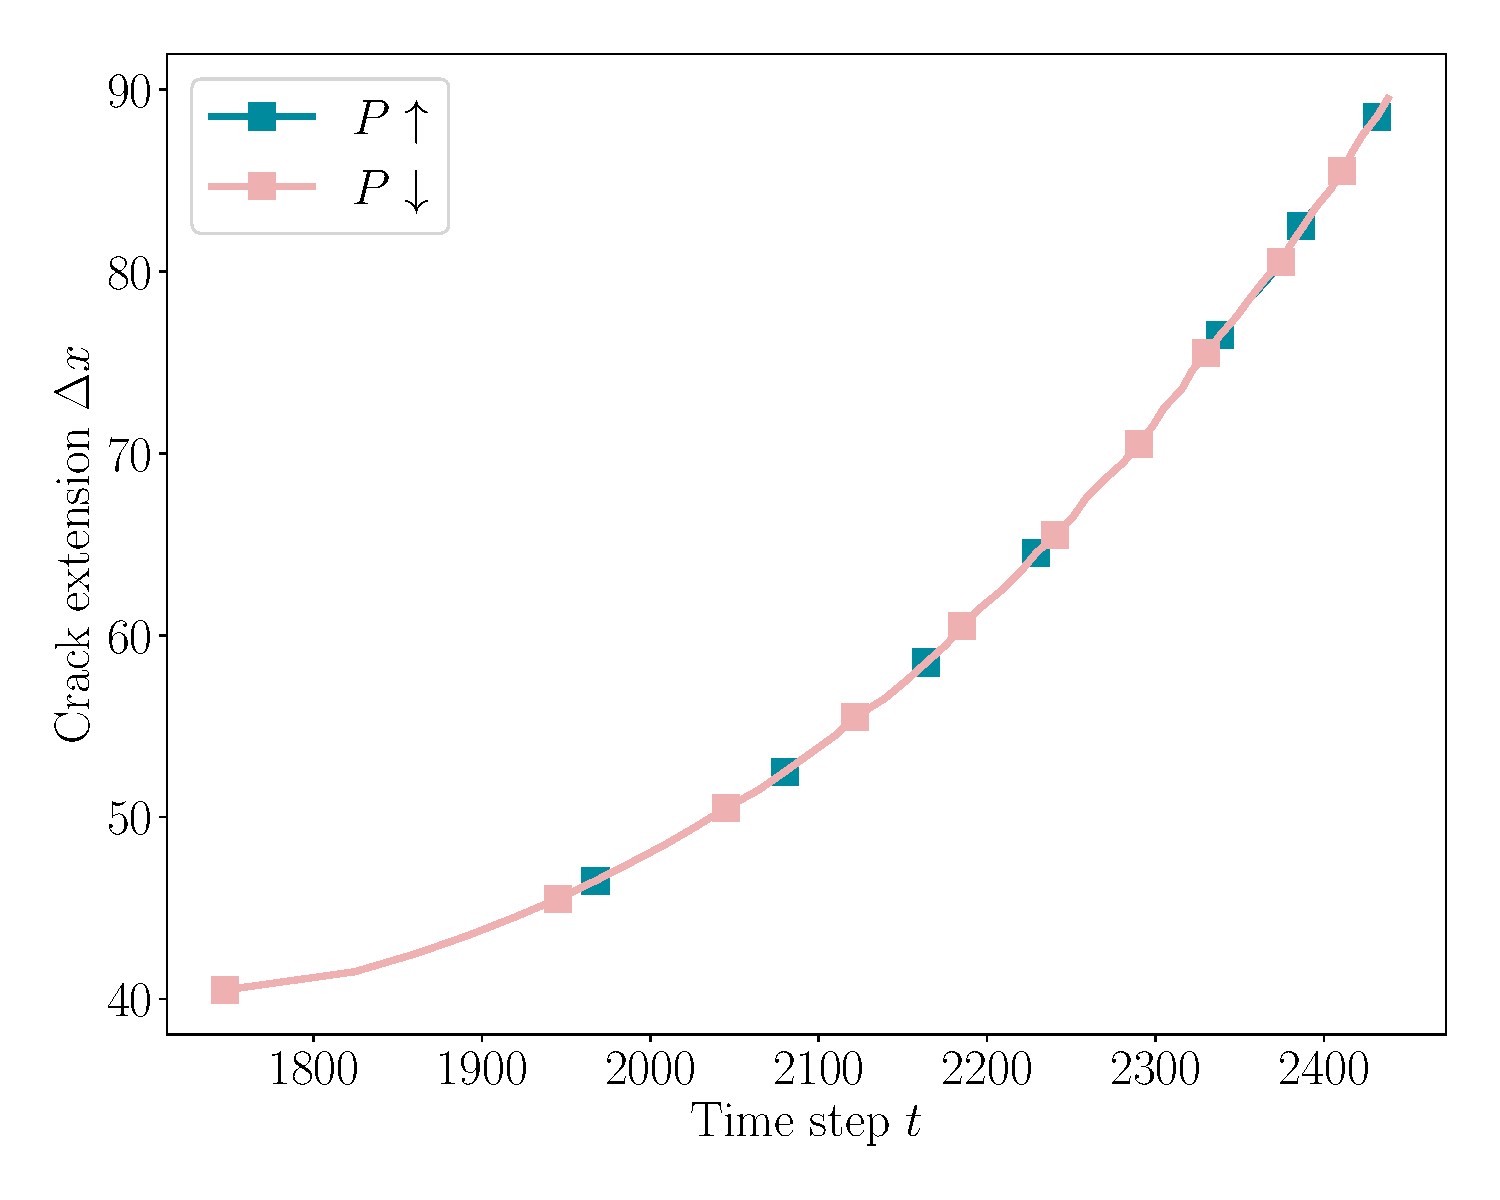
\includegraphics[width=0.55\linewidth]{FigS4.pdf}
    \caption{The change in crack extension length over time step $t$. Arrows in the figure indicate the direction of initial polarization.} \label{figS4}
\end{figure}
\end{enumerate}
\end{response}
\newpage
\begin{question}{\QuestionRevA{Q6}}\label{R1:Q6}
Figure 2 shows domain patterns very similar to the simulations in Li (2011) http://hdl.handle.net/2152/ETD-UT-2011-12-4705 (also see Li and Landis (2011) Eng. Frac. Mech 78, 1505-1513 for a publication with the electrical case). It would be useful if this work were referenced as a comparison.
\end{question}

\begin{response}
Thanks for your constructive comment. We appreciate the reference to the work by Li (2011) and the subsequent publication by Li and Landis (2011) in Engineering Fracture Mechanics. These references indeed provide valuable comparisons to our domain patterns.

We have included both references in the revised manuscript as:

On page 20, 
\begin{revised}
Similar domain evolution process near the crack tip are also reported by Wang et al. [21] \textcolor{blue}{and Li et al. [60, 61]}.  (Ref. 60 and 61 is the research from Li et al.)
\end{revised}
\end{response}

\begin{question}{\QuestionRevA{Q7}}\label{R1:Q7}
    "Crack" is spelled "Creack" on several of the Figures. Please check and correct these.
\end{question}
\begin{response}
Thanks for your carefully reading and constructive comments. We are sorry for the typos in the manuscript. In the revised manuscript, we have corrected these typos on Fig. 4(a), Fig. 7(a) and Fig. 11(a).
\end{response}

\begin{question}{\QuestionRevA{Q8}}\label{R1:Q8}
It's unclear what the dimensionless ratios are that are being reported in Table 1. Specifically, is the kappa in Table 1 consistent with the permittivity of free space? If not then it is not being defined properly.
\end{question}
\begin{response}
We are really appreciate for the comment. The dimensionless ratios in Table 1 are referenced from our previous work (Liu et al., IJSS, 162, 198–210, 2019). We apologize for any confusion caused by not providing explicit formulas in the paper. To clarify, we have included the dimensionless formulas for each parameter in the supplementary material. For the dielectric constant $\kappa$, as the reply to comment 1, it should be the relative permittivity of the background material.

In the revised manuscript, the following equations are added on page 16:
\begin{revised}
In the simulation, dimensionless parameters are utilized to ensure computational accuracy[48]:
\setcounter{equation}{47}
\textcolor{blue}{
\begin{equation}
    \begin{split}
        & \mathbf{x}^*=\sqrt{|\alpha_0|/G_{110}}\mathbf{x}, \quad
        \mathbf{P}^*=\mathbf{P}/{P_0}, \quad
        \mathbf{\kappa^*}=\kappa |\alpha_0|, \quad
        \alpha_1^*=\alpha_1/|\alpha_0|, \quad \\
        & t^*=|\alpha_0 | L_P t, \quad
         \alpha_{ij}^*=\alpha_{ij}P_0^2/|\alpha_0|, \quad
        \alpha_{ijk}^*=\alpha_{ijk}P_0^4/|\alpha_0|, \quad
        Q_{ij}^*=Q_{ij}P_0^2, \quad \\
       &c_{ij}^*=c_{ij}/(|\alpha_0|P_0^2),\quad
        G_{ij}^*=G_{ij}/G_{110}, \quad
       f_{ij}^*=f_{ij}\sqrt{|\alpha_0|/G_{110}}/(|\alpha_0| P_0), \quad
    \end{split}
\end{equation}
where $\alpha_0=1.73\times 10^8$ $\text{m}^2 \text{N/C}^{-2}$ denotes the value of $\alpha_1$ at $25 ~^\circ $C, $G_{110}= 1.73\times 10^{-10}$ $\text{m}^4 \text{N/C}^{-2}$ is the reference value of the gradient energy coefficient, and $P_0=0.76$ $\text{C/m}^{2}$  is the spontaneous polarization of \ce{PbTiO3} at room temperature.}
\end{revised}
\end{response}

\begin{question}{\QuestionRevA{Q9}}\label{R1:Q9}
    Can the authors comment on the two kinetic coefficients? Is it being assumed that crack propagation happens faster than domain growth? Is there justification for this?
\end{question}
\begin{response}
    Thank you very much for your constructive comments. In the current model, the time scales of these three processes are characterized by two mobility coefficients $L_P$ and $L_\nu$. The larger the mobility coefficient is, the faster the process evolves (Charlotte, EFM, 77.18, 3625-3634, 2010).  In this study, the time is normalized according to the polarization mobility coefficient $L_P$. The chosen value of $L_p$ is $4.0\times10^4$ $\text{N}^{-1}\text{C}^2\text{m}^{-2}\text{s}^{-1}$, which is estimated by the experimental observation of domain switching in ferroelectric materials and widely used in the ferroelectric phase field community (Tomas, Nat. Comm., 3.1, 748, 2012). On the determination of $L_\nu$, it is estimated by the ranges of the crack velocities ($10^2-10^3$m/s) in experiments, which is also adopted by Zhang et al. (Zhang, IJMS, 236, 107747, 2022). The relatively small mobility of the crack field allows us to capture both the crack propagation and domain evolution in the simulation, which is also employed by Abdollahi et al (Abdollahi, Acta Mater., 59.12, 4733-4746, 2011; Abdollahi, JMPS, 60.12, 2100-2126, 2012).

    In the revised manuscript, the following sentences is added on page 17:
    \begin{revised}
        \textcolor{blue}{The normalized time is determined by $L_P=4.0\times10^4$ $\text{N}^{-1}\text{C}^2\text{m}^{-2}\text{s}^{-1}$. $L_\nu$ is estimated to recover the magnitude of the crack extension speed. The relatively small mobility of the crack field can help capture both the crack propagation and domain evolution in the simulation [29, 31].}
    \end{revised}
\end{response}

\begin{question}{\QuestionRevA{Q10}}\label{R1:Q10}
Can the authors also comment on the domain wall width and fracture process zone length scales? Are they physically comparable? How do they compare to the mesh size chosen?
\end{question}
\begin{response}
Thanks for your comments. The domain wall width is characterized by the gradient energy coefficient. The normalized unit length represents 1.0 nm according to the chosen reference polarization gradient energy coefficient $G_110=1.73×10^{-10}$ $\text{Nm}^4\text{C}^{-2}$. The simulated domain wall thickness is about 1 unit length with the \ce{PbTiO3} gradient energy coefficients, which are verified to be reasonable by experimental results (Stemmer,Solid state ionics 75, 43-48, 1995; Li, J. Appl. Phys., 98, 064101, 2005). In our simulation, the largest element size is 2×2. Since we employ the 3rd-order PHT-mesh in the calculation, each boundary of the element is divided by 4 nodes. Thus, it is sufficient to ensure the accuracy.

For the diffuse interface of crack, its thickness is characterized by the internal fracture length parameter. Initially, the length parameter is introduced as a numerical parameter to facilitate the solution using numerical methods and to prevent any mesh dependence of the crack path. Later, this parameter is also viewed as a physical or material parameter related to material’s internal length or intrinsic strength by some researchers. As illustrated by Amor et al. (Amor, JMPS, 57.8, 1209-1229, 2009), the value of the length parameter may be chosen according to two different points of view, depending on whether it is considered as a pure numerical parameter of the regularized fracture model or as a real physical material parameter of a gradient damage model. In the latter case, the length parameter value must be selected according to experimental data or some material characteristic length.

Since there is limited the experimental data for the situation, the correlation between the length scale and the size of the fracture process zone is still an open issue. As a result, we consider the length parameter as a pure numerical parameter. It should cover several finite elements to ensure a smooth description of the diffuse crack interface. Meanwhile, it should smaller enough to give a close convergence to the corresponding sharp interface theory (Bourdin, Journal of Elasticity 91, 5-148, 2008). In our simulation, the dimensions value of $l_v$ is set to be 1, and the calculated thickness of crack is about 1 unit length, which is larger than the length of the refined element. 
\end{response}

\begin{flushleft}
    \vspace{1em} 
    \hrule
    \vspace{1em} 
    \textbf{Point-by-point Reply to Reviewer2}
    \vspace{1em} 
    \hrule
    \vspace{1em} 
\end{flushleft}
\begin{question}{\QuestionRevB{General}}
This work presents a phase-field model for ferroelectric materials to analyze the fracture and domain behavior due to flexoelectric effects. Both direct and converse flexoelectric effects are considered in the formulation and the governing equations are further solved using PHT-spline.
\end{question}
\begin{response}
    First, we would like to express our sincere gratitude to you for your careful reading and evaluating our manuscript. We also thank you for your interest, constructive comments, and recommendations. We answer all your comments and revise the manuscript accordingly as follows.
\end{response}

\begin{question}{\QuestionRevB{Q1}}\label{R2:Q1}
    However, I see a major flaw in the formulation: the strain gradient elasticity is not considered at all in the formulation. Please see your equation (1), the sixth order gradient elasticity tensor that couples strain-gradient with strain-gradient is missing. Note that such gradient elastic effects will change the overall stiffness of the material and as a result the fracture and its progression will be changed.
\end{question}
\begin{response}
    Thanks for your carefully reading and constructive comments. Rigorously speaking, the strain gradient energy $\psi_{grad-\varepsilon}$ should be considered in the formulation of total energy density. Jiang et al. has detailed discussed the influence of $\psi_{grad-\varepsilon}$ on ferroelectric materials (Jiang, JAP, 120, 234102, 2016). Their results show that the $\psi_{grad-\varepsilon}$ contributes to the stabilization and smooth distribution of domain morphology.  Yet, $\psi_{grad-\varepsilon}$ is often ignored in the research of flexoelectric effect in ferroelectrics. There are mainly two reasons: 1. the sign and magnitude of strain gradient energy coefficient is still disputed (Eliseev, PRB, 97, 2, 024102, 2018); 2. the impact of $\psi_{grad-\varepsilon}$ on the electromechanical properties of ferroelectrics is insignificant when $f_{klmn}^2<G_{ijkl} c_{ijmn}$. Here, $G_{ijkl}$ and $c_{ijmn}$ is the gradient energy coefficient and elastic stiffness, respectively (Eliseev, PRB, 79, 16, 165433, 2009; Chen, JMPS, 79, 108-133, 2015; Xu, SMS,  26, 11, 115024). Since we mainly focus on the flexoelectric effect, an extended discussion on strain gradient energy is beyond the scope of this study. Therefore, we decide to ignore the strain gradient energy in our calculations. 

    Based on your valuable suggestions and to facilitate understanding, we have added the following content in the revised manuscript:
    \begin{enumerate}
    \item In Eq.(1),
    \setcounter{equation}{0}
    \begin{revised}
        \begin{equation}
            \psi(\mathbf{\varepsilon},\nabla\mathbf{\varepsilon},\phi,\mathbf{P},\nabla\mathbf{P})
            =\psi_\mathrm{Land}+\textcolor{blue}{\psi_\mathrm{grad-P}}+\psi_\mathrm{elas}+\psi_\mathrm{flex}\textcolor{blue}{+\psi_\mathrm{grad-\varepsilon}}+\psi_\mathrm{elec},
        \end{equation}
    \end{revised}
        \item The following paragraph is added after Eq.(6),
        \setcounter{equation}{7}
        \begin{revised}
        \textcolor{blue}{
            Due to the size effect, giant strain gradient can be easily generated at nanoscale. According to Mindlin's strain-gradient elastic theory, the strain gradient energy should also be included at nanoscale  [38], which can be written as:
\begin{equation}
    \psi_\mathrm{grad-\varepsilon}=\frac{1}{2}\nabla\mathbf{\varepsilon}\,\vdots\,\mathbb{W}\,\vdots\,\nabla\mathbf{\varepsilon},
\end{equation}
in which $\mathbb{W}$ denotes the strain gradient energy coefficient. In ferroelectric materials, $\psi_\mathrm{grad-\varepsilon}$ promotes the stabilization of the domain morphology when the flexoelectric coefficients exceed the upper boundaries, namely $f_{klmn}^2>G_{ijkl}c_{ijmn}$ [39]. Nevertheless,  $\psi_\mathrm{grad-\varepsilon}$ can be neglected when $f_{klmn}^2<G_{ijkl}c_{ijmn}$ [40-42]. Besides, the magnitude and sign of $\mathbb{W}$ are still controversial. For the reasons mentioned above, $\psi_\mathrm{grad-\varepsilon}$ is omitted in the following sections.}
        \end{revised}
    \end{enumerate}
\end{response}
\begin{question}{\QuestionRevB{Q2}}\label{R2:Q2}
 Further, the authors have not provided constitutive relations, for instance, see equation 18: how is $\tau$ related to $\nabla\varepsilon$? This should be provided in the same Section.
\end{question}
\begin{response}
We are really appreciating for the comment. We are sorry for the inconvenience in obtaining the constitutive relations from Eqs.(18)-(19). In the revised manuscript, we have provided the full expression of the constitutive relations:
\setcounter{equation}{18}
\begin{revised}
    The constitutive equations of each physical field can be derived from the total enthalpy density $\psi_\mathrm{t}$:
\textcolor{blue}{
\begin{equation}
    \sigma_{ij}=\frac{\partial\psi_t}{\partial\varepsilon_{ij}}=g(\nu)\left( c_{ijkl}\varepsilon_{kl}-q_{ijkl}P_kP_l \right),
\end{equation}}
\textcolor{blue}{
\begin{equation}
    \tau_{ijl}=\frac{\partial \psi_\mathrm{t}}{\partial \varepsilon_{ij,l}}=-\frac{1}{2} g(\nu)\left( f_{ijkl} P_k \right),
\end{equation}
\begin{subequations}
    \begin{equation}
        \begin{split}
            \eta_i&=\frac{\partial\psi_\mathrm{t}}{\partial P_i}=\alpha_{ij}P_j+\alpha_{ijkl}P_jP_kP_l+\alpha_{ijklmn}P_jP_kP_lP_mP_n \\
             &-g(\nu)\left( q_{ijkl}P_j\varepsilon_{kl}+\frac{1}{2}f_{ijkl}\varepsilon_{kl,j} \right)-E_i,\quad \text{(electrically permeable)}
        \end{split}
    \end{equation}
    \begin{equation}
        \begin{split}
            \eta_i&=\frac{\partial\psi_\mathrm{t}}{\partial P_i}=\alpha_{ij}P_j+\alpha_{ijkl}P_jP_kP_l+\alpha_{ijklmn}P_jP_kP_lP_mP_n \\
         &-g(\nu)\left( q_{ijkl}P_j\varepsilon_{kl}+\frac{1}{2}f_{ijkl}\varepsilon_{kl,j}+E_i\right),\quad \text{(electrically impermeable)}
        \end{split}
    \end{equation}
\end{subequations}
\begin{equation}
    \Lambda_{ij}=\frac{\partial \psi_\mathrm{t}}{\partial P_{i,l}}=g(\nu)\left( G_{iljk}P_{j,k}-\frac{1}{2}f_{ijkl}\varepsilon_{jk} \right),
\end{equation}
\begin{subequations}
    \begin{equation}
        D_i=-\frac{\partial \psi_\mathrm{t}}{\partial E_i}=\kappa E_i+P_i, \quad \text{(electrically permeable)}
    \end{equation}
    \begin{equation}
        D_i=-\frac{\partial \psi_\mathrm{t}}{\partial E_i}=g(\nu)(\kappa E_i+P_i), \quad \text{(electrically impermeable)} 
    \end{equation}
\end{subequations}}
\end{revised}
\end{response}

\begin{question}{\QuestionRevB{Q3}}
Pg 4 "gradient energy tensor": please see the literature for its correct name.
\end{question}

\begin{response}
Thanks for your carefully reading. We are sorry for the incorrect description about $\mathbb{G}$. It should be named as "gradient energy coefficients". In the revised manuscript, this issue is addressed:
    \begin{revised}
        ... where $\mathbb{G}$ is the $4^\mathrm{th}$-rank gradient energy \textcolor{blue}{coefficients}.
    \end{revised}
\end{response}

\begin{question}{\QuestionRevB{Q4}}
Pg 5: Spelling "donating".
\end{question}
\begin{response}
We highly appreciate you for your careful reading. We are sorry for the typo. In the revised manuscript, the tpyo is corrected:
\begin{revised}
    ... with $\mathbb{C}$ \textcolor{blue}{denoting} the elastic stiffness tensor...
\end{revised} 
\end{response}

\begin{question}{\QuestionRevB{Q5}}
Citation to Equation (9) is missing.
\end{question}
\begin{response}
    Thanks for your valuable comment. The expression of $\psi_{frac}$ is primarily based on the work of Miehe et al. (IJNME, 83, 10, 1273–1311, 2010), which is cited as Ref. [40] in the original manuscript. We apologize for not providing the citation in the correct location and have made the necessary corrections in the revised manuscript:

    On page 6 of the revised manuscript:
    \begin{revised}
        ... and $\psi_\mathrm{frac}$ represents the fracture energy related to the energy dissipation in creating the crack surface \textcolor{blue}{[48]}:
    \end{revised}
    Ref. [48] is the research of Miehe et al. (IJNME, 83, 10, 1273–1311, 2010). 
\end{response}

\begin{question}{\QuestionRevB{Q6}}
    "To investigate the crack evolution in ferroelectrics, it is necessary to determine the coupling relationship among the crack and other physical fields, such as strain $\varepsilon$, electric field E, and polarization P": What about gradP and gradE?
\end{question}
\begin{response}
    We highly appreciate you for your important comments. As you mentioned, the crack field is indeed coupled with $\nabla \mathbf{P}$ and $\nabla \varepsilon$. However, crack propagation is independent of $\nabla \mathbf{E}$ since we do not consider $\nabla \mathbf{E}$ here. To clarify, we have made the following corrections in the revised manuscript:

    On page 7 of the revised manuscript,
    \begin{revised}
        ... such as strain $\mathbf{\varepsilon}$, \textcolor{blue}{strain gradient $\nabla \varepsilon$,} electric field $\mathbf{E}$, polarization $\mathbf{P}$, \textcolor{blue}{and polarization gradient $\nabla \mathbf{P}$}. 
    \end{revised}
\end{response}

\begin{question}{\QuestionRevB{Q7}}
    Pg7: Check inverted commas and remove repetition of "In this study".
\end{question}
\begin{response}
    Thanks for your careful reading. We have corrected the inverted commas. The repetition of "In this study" before Eq.(12) is removed in the revised manuscript. 

    On page 7 of the revised manuscript:
    \setcounter{equation}{11}
    \begin{revised}
        Due to the symmetry breaking at the crack surface, the polarization is influenced by the surface effect. \textcolor{blue}{In this study}, the free-polarization boundary condition is applied on the crack surface:
        \begin{equation}
            \frac{\mathrm{d}P_i^+}{\mathrm{d}\mathbf{n}^+}=\frac{\mathrm{d}P_i^-}{\mathrm{d}\mathrm{\mathbf{n}^-}}=0,
        \end{equation}
        where the superscripts \textcolor{blue}{``+''} and \textcolor{blue}{``-''} indicate the upper and lower surfaces of the crack, respectively.
    \end{revised}
\end{response}

\begin{question}{\QuestionRevB{Q8}}
    Paragraph above Eq. 22: change "external stress" to external force. You cannot apply external stress.
\end{question}
\begin{response}
    Thanks for your constructive suggestion. According to your comment, we have made the following changes in the revised manuscript:

    On page 10, 
    \begin{revised}
        ... When subjected to external \textcolor{blue}{force} or electric fields, the domain morphology will evolve with the motion and nucleation of domain walls...
    \end{revised}
\end{response}

\begin{question}
    {\QuestionRevB{Q9}}
    Eqn 28: check the subscript.
\end{question}
\begin{response}
    Thanks for pointing out the typos. We have corrected the subscript in the revised manuscript:

    On page 11,
    \setcounter{equation}{32}
    \begin{revised}
        Then, the elastic energy can be decomposed as:
    \begin{equation}
    \textcolor{blue}{\psi_\mathrm{elas}}=\textcolor{blue}{\psi_\mathrm{elas}^+}+\textcolor{blue}{\psi_\mathrm{elas}^-},
    \end{equation}
    \end{revised}
\end{response}

 \begin{question}
     {\QuestionRevB{Q10}}
     Section 3.1: remove extra period sign after [48].
 \end{question}
 \begin{response}
     Thanks for your careful reading. In the revised manuscript, we have addressed this issue:

     On page 13,
     \begin{revised}
         ... The polynomial splines over hierarchical T-meshes (PHT-spline) are adopted as the basis function to achieve high-order continuity [57]. \textcolor{blue}{Compared} to the commonly used non-uniform rational B-spline (NURBs) in IGA, ...
     \end{revised}
 \end{response}

\end{document}